%=====================================================================
\section{Survival of wall defects and docking in circles}\label{sec:csurv}
Two complementary measures (methods: Secs.~\ref{sec:md-labels}, \ref{sec:m-surv}). \emph{Label survival} follows the wall
defects present at a reference time, passing the label to the birth partner when a wall defect annihilates; it asks whether
the wall defects stay at the wall, whoever they are. \emph{Visit survival} follows each $+\half$ track and measures how long it
stays once it has reached the wall (Kaplan--Meier with censoring), plus the reverse process, docking of bulk $+\half$.
\begin{figure}[H]\centering
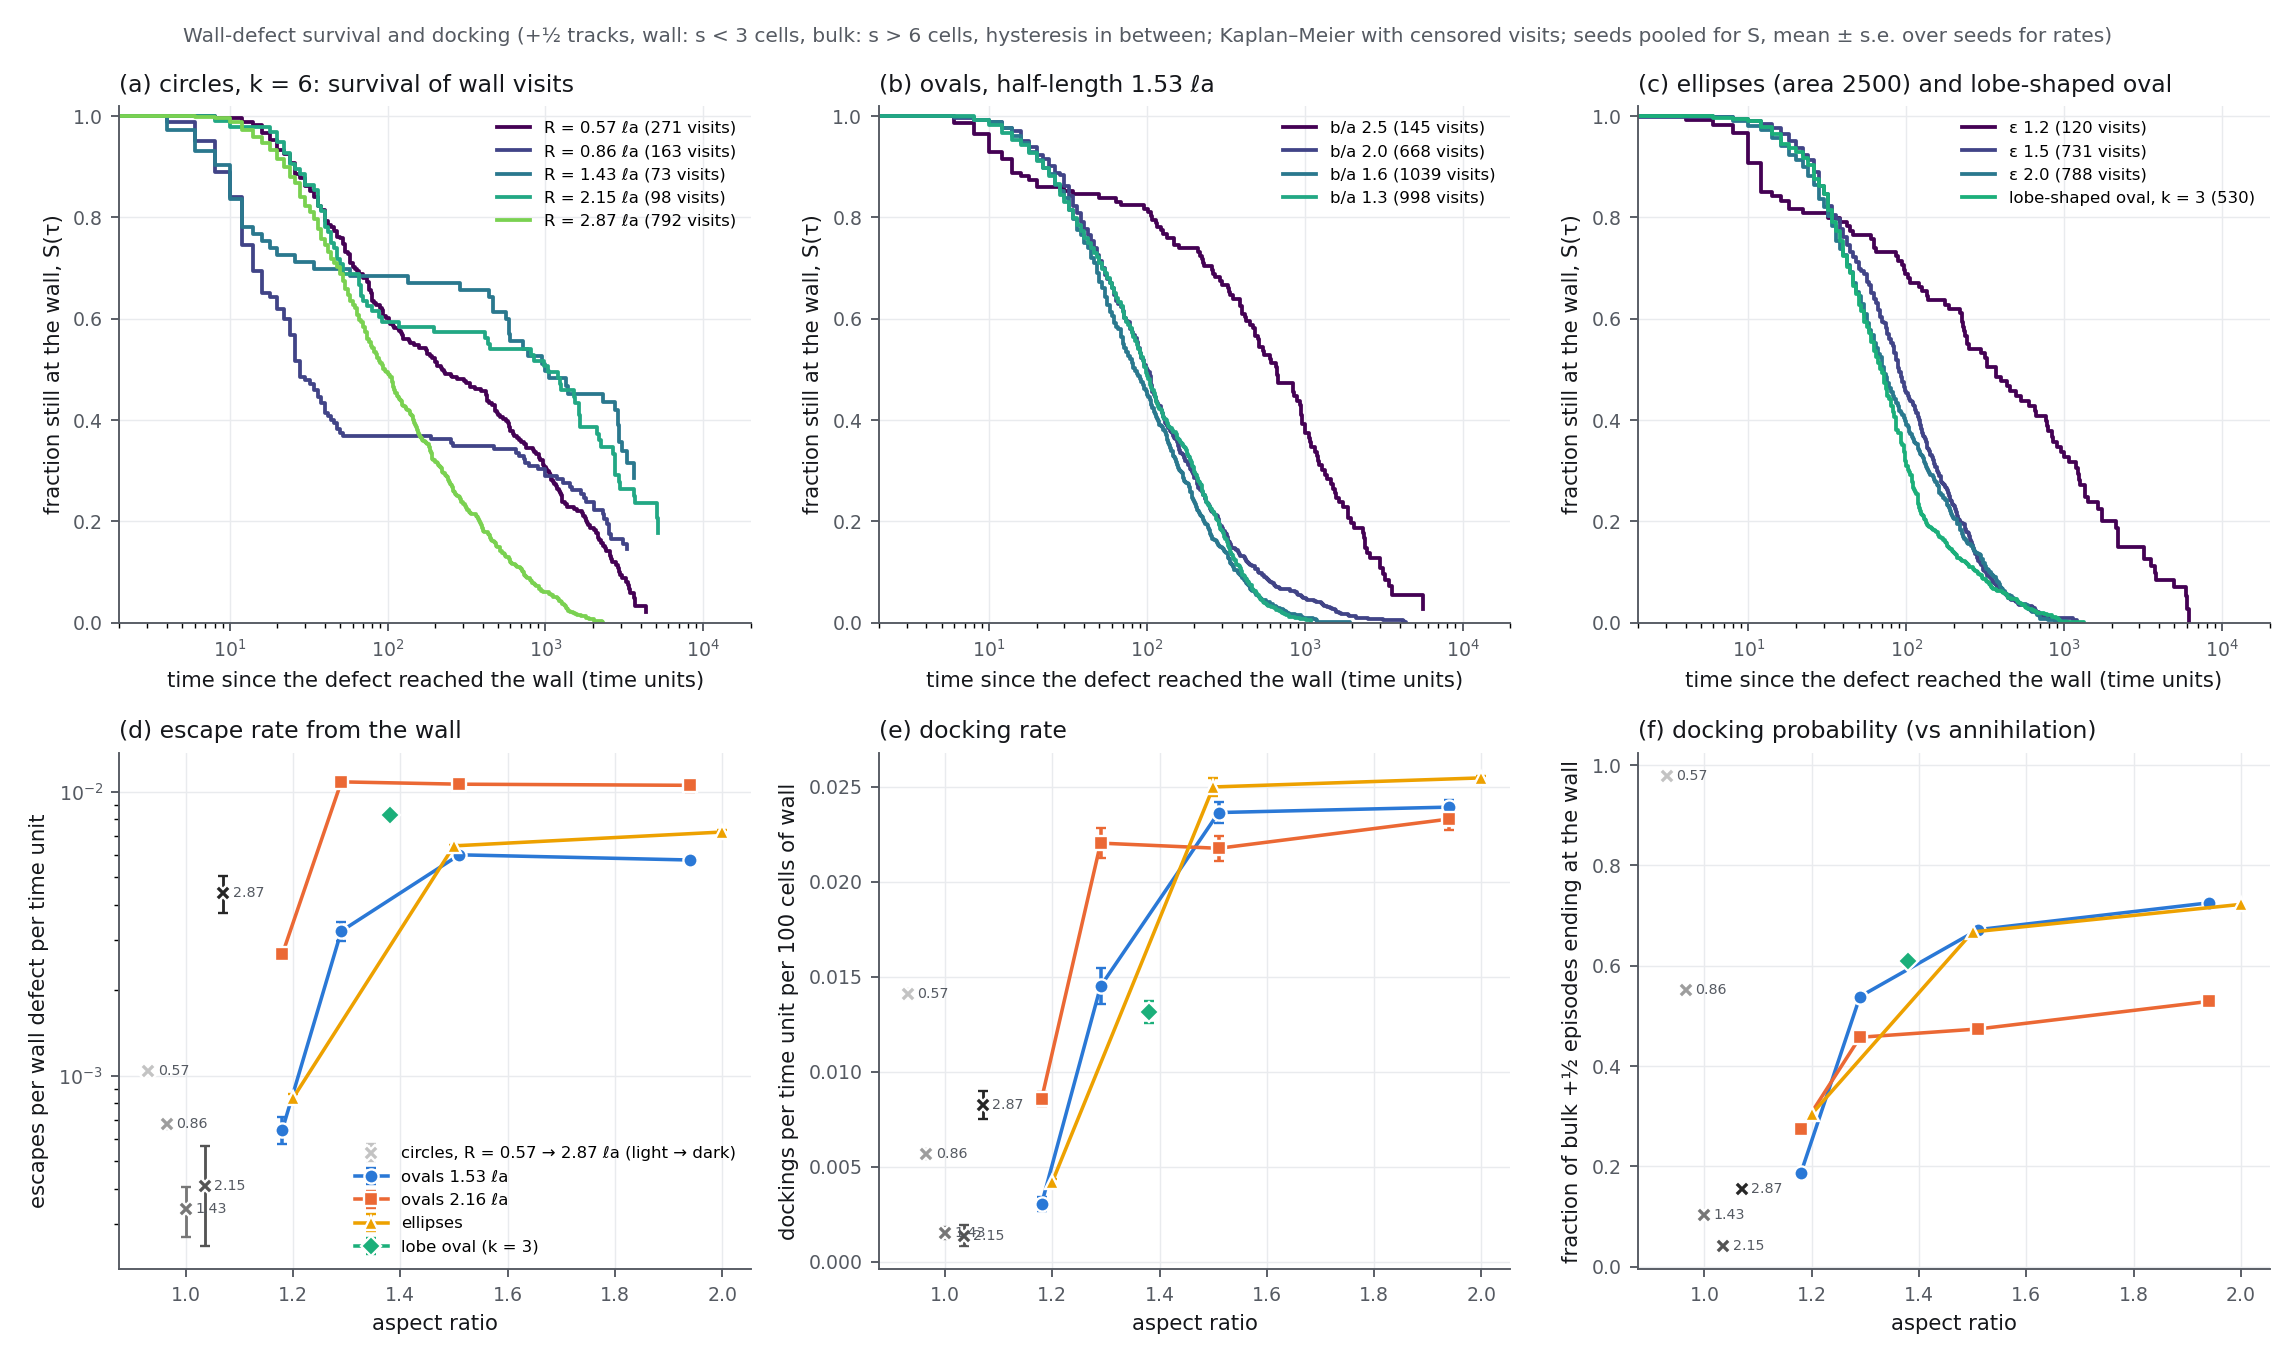
\includegraphics[width=\textwidth]{survival_docking.png}
\caption{\textbf{Survival and docking.} (a--c) Kaplan--Meier survival $S(\tau)$ of wall visits for circles ($k=6$, five sizes),
ovals of half-length $1.53\,\la$, ellipses and the lobe-shaped oval (seeds pooled; numbers of visits in the legends).
(d) Escape rate per wall defect, (e) docking rate per 100 cells of wall, (f) fraction of bulk $+\half$ episodes that end at
the wall rather than by annihilation; mean $\pm$ s.e.\ over seeds, against the aspect ratio (circles at aspect 1, light to dark
= $R=0.57\to2.87\,\la$). Wall: $s<3$ cells, bulk: $s>6$ cells.}\label{fig:surv}
\end{figure}
\begin{figure}[H]\centering
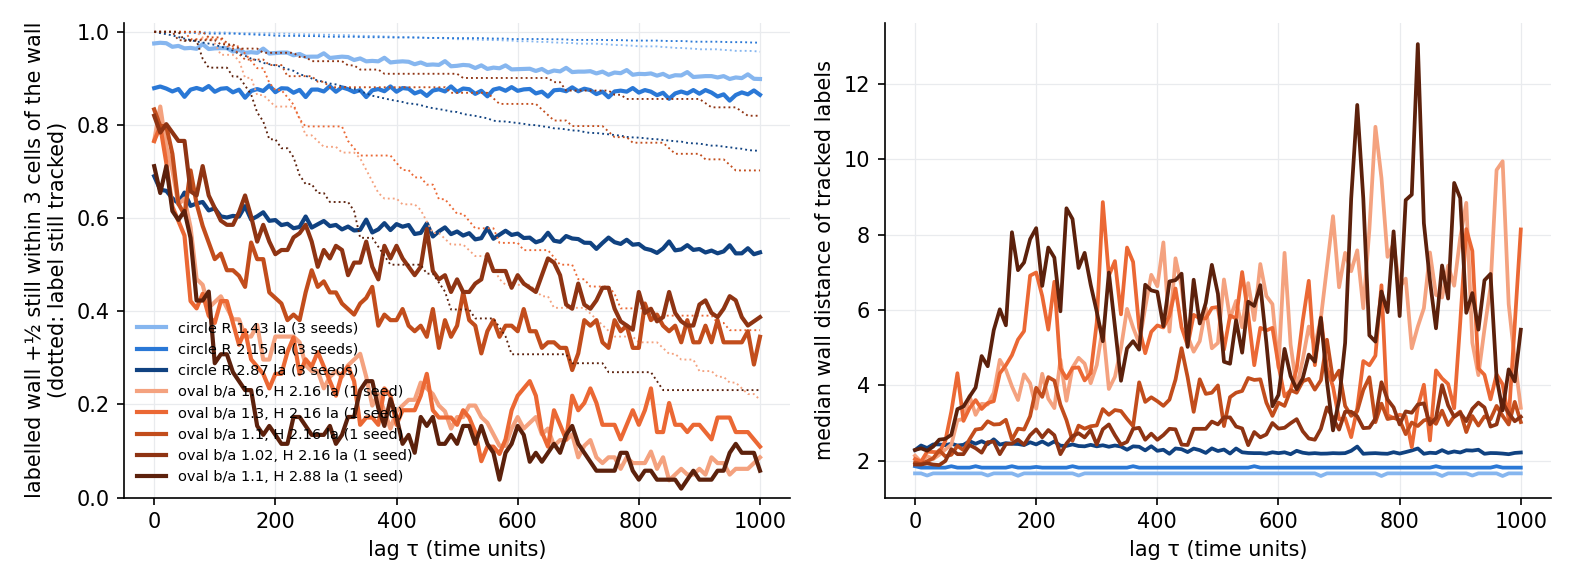
\includegraphics[width=\textwidth]{labels_circles_ovals.png}
\caption{Label survival: fraction of the labelled wall defects within 3 cells of the wall (left) and median wall distance of
tracked labels (right) against the time since labelling, circles ($k=6$, 3 seeds per size) and ovals (half-length 2.16 and
$2.88\,\la$, 1 seed).}\label{fig:labels}
\end{figure}
\begin{table}[H]\centering\small
\caption{Circles, $k=6$, 3 seeds: wall-visit survival and docking (\texttt{reports/master/data/survival\_docking.txt}).
Visits: wall visits with observed start; $t_{1/2}$: time at which $S=\half$ (time units); docking rate per 100 cells of wall per time unit; bulk time: median time in the bulk before docking.}\label{tab:csurv}
\begin{adjustbox}{max width=\textwidth}
\begin{tabular}{lcccccccc}\toprule
$R/\la$ & visits & wall $+\half$ & escape rate ($10^{-3}$) & $S(1000)$ & $t_{1/2}$ & docking rate & $P_\mathrm{dock}$ & bulk time\\\midrule
0.57 & 271 & 10.9 & $1.04\pm0.02$ & 0.31 & 220 & 0.014 & 0.98 & 72\\
0.86 & 163 & 10.1 & $0.67\pm0.02$ & 0.29 & 28 & 0.006 & 0.55 & 76\\
1.43 & 73 & 10.0 & $0.34\pm0.07$ & 0.50 & 1000 & 0.0015 & 0.10 & 25\\
2.15 & 98 & 9.9 & $0.41\pm0.16$ & 0.51 & 1044 & 0.0014 & 0.04 & 21\\
2.87 & 792 & 8.4 & $4.4\pm0.7$ & 0.06 & 96 & 0.008 & 0.15 & 24\\\bottomrule
\end{tabular}
\end{adjustbox}
\end{table}
\begin{itemize}
  \item \textbf{In clean circles the wall defects stay.} At 1.43 and $2.15\,\la$ half of the wall visits last longer than 1000
        time units, and a wall defect escapes about once per 3000 time units (escape rate $3$--$4\times10^{-4}$). Label survival:
        84--94\% of the labelled wall defects are still at the wall after 1000 time units; the median wall distance of tracked labels
        stays at 1.7--2.3 cells. The few visits in these runs (73--98) are because the layer barely exchanges.
  \item \textbf{Docking is rare:} only 4--10\% of bulk $+\half$ excursions end at the wall; the rest end by annihilating with a
        $-\half$ in the bulk. The $2k-2$ layer and the bulk are almost decoupled populations.
  \item \textbf{Large circle ($2.87\,\la$):} escape rate 13$\times$ higher, $S(1000)=0.06$; labels 41--59\% at the wall after 1000.
        This is the degraded layer of Sec.~\ref{sec:sweep}: vacancies (occupancy 0.78), upstream drift (Sec.~\ref{sec:clattice}) and
        exchange.
  \item \textbf{Small circles} ($\le0.86\,\la$) are a different regime: no or few bulk pairs (0 and 0.4 $-\half$ per frame), and
        the cavity is only a few wall-to-bulk thresholds across, so $+\half$ cross the 3/6-cell thresholds often, visits are short and
        docking is frequent ($P_\mathrm{dock}=0.55$--0.98). The wall lattice is weakly pinned at $0.57\,\la$ (static fraction 0.51)
        and mostly pinned at $0.86\,\la$ (0.83).
  \item The layer empties, when it does, by undocking: at most 10\% of wall visits end in annihilation (exchange analysis).
\end{itemize}
\open{The docking pathway itself (H7: do bulk $+\half$ circulate along the layer edge and insert into the largest gaps?) has not
been analysed yet; the tracks needed for it exist.}
